\section{Resultados}

\subsection{Calibração da XRF}

\begin{frame}
  \frametitle{}
  \begin{figure}
      \centering
      \includegraphics[width=0.5\linewidth]{../../outputs/CalibrationK2010MaiAkerr.pdf}
      \includegraphics[width=0.5\linewidth]{../../outputs/CalibrationL2010MaiAkerr.pdf}
  \end{figure}
\end{frame}

\begin{frame}
  \frametitle{}
  Comparação das calibrações da XRF-ED nos 3 períodos.
  \begin{figure}[H]
    \begin{subfigure}[b]{0.5\textwidth}
      \includegraphics[width=\textwidth]{../../outputs/CalibrationKcomparacao.pdf}
      \caption{linha K}
    \end{subfigure}%
    \begin{subfigure}[b]{0.5\textwidth}
      \includegraphics[width=\textwidth]{../../outputs/CalibrationLcomparacao.pdf}
      \caption{linha L}
    \end{subfigure}
  \end{figure}
\end{frame}


\begin{frame}
  \frametitle{}
  Comparação das análises de XRF no LAPAt e na US-EPA. 
  \begin{figure}[H]
    \centering
      \includegraphics[width=0.3\textwidth]{../../outputs/epa_iag_S.pdf}
      \includegraphics[width=0.3\textwidth]{../../outputs/epa_iag_K.pdf}
      \includegraphics[width=0.3\textwidth]{../../outputs/epa_iag_Ca.pdf}
  \end{figure}
\end{frame}


\begin{frame}
  \frametitle{}
  \begin{figure}[H]
    \centering
      \includegraphics[width=0.3\textwidth]{../../outputs/epa_iag_P.pdf}
      \includegraphics[width=0.3\textwidth]{../../outputs/epa_iag_Cl.pdf}
      \includegraphics[width=0.3\textwidth]{../../outputs/epa_iag_V.pdf}
  \end{figure}
\end{frame}

\subsection{Black Carbon}
\begin{frame}
  \frametitle{}
  \begin{figure}[H]
    \centering
    \includegraphics[width=0.9\textwidth]{../../outputs/BC_monarch71.pdf}
    \caption{Calibração do refletômetro do LAPAt em 2007 usando alvos padrões M71.
           \label{fig:monarch71}}
  \end{figure}
\end{frame}


\begin{frame}
  \frametitle{}
  \begin{figure}[H]
  	\centering
  	\includegraphics[width=0.7\linewidth]{../../outputs/BC_cetesb.pdf}
  	\caption{Reflêtancia e pesagem dos padrões produzidos na CETESB com BC 
                   de referência ASTM-N762. \label{fig:bc_cetesb}}
  \end{figure}
\end{frame}


\begin{frame}
  \frametitle{}
  \begin{figure}[H]
    \centering
    \includegraphics[width=0.5\linewidth]{../../outputs/JQ_TOT_Refletancia.pdf}
    \caption{Intercalibração TOT e Reflêtancia para amostragem paralela no 
             túnel Jânio Quadros. \label{table:interJQ}}
  \end{figure}
\end{frame}


\begin{frame}
  \frametitle{}
  Comparação da massa de BC das amostras do túnel Jânio Quadros 
                 calculada usando calibração por TOT(1) versus calibração a partir dos 
                 alvos padrões produzidos na CETESB(2)
  \begin{figure}[H]
    \centering
      \includegraphics[width=0.6\linewidth]{../../outputs/BC_janio_quadros.pdf}

  \end{figure}
\end{frame}


\begin{frame}
  \frametitle{}
  \begin{figure}[H]
  	\begin{center}
  		\includegraphics[width=0.9\textwidth]{../../outputs/Gana_TOT_Refletancia.pdf}
  		\caption{Intercalibração entre TOT e refletância em Acra. \label{fig:interGanaBC}}
  	\end{center}
  \end{figure}
\end{frame}

\begin{frame}
  \frametitle{}
  Razão dos valores de BC medidos por refletância e calibrados por 
  TOT e M71 para Recife e Acra.
  \begin{figure}[H]
  	\centering
  	\begin{subfigure}[b]{0.43\linewidth}
  		\includegraphics[width=\linewidth]{../../outputs/BC_compara_calibs.pdf}
  		\caption{Acra \label{fig:razaoTOTM71}}
  	\end{subfigure}
  		\hspace{0.3cm}
  	\begin{subfigure}[b]{0.43\linewidth}
  		\includegraphics[width=\linewidth]{../../outputs/BC_compara_calibs_recife.pdf}
  		\caption{Recife \label{fig:BC_compara_recife}}
  	\end{subfigure}%
   \end{figure}
\end{frame}

\begin{frame}
  \frametitle{}
 % Padrões de Qualidade do Ar para $MP_{10}$ Ambiental em Gana
  \begin{table}[H]
  \centering
  \tiny 
    % http://www.epa.gov.gh/ghanalex/policies/EPAguidelines%20Report.pdf
\begin{tabular}{cccc}
\hline
                              &   regiões  &        zonas       &         zonas               \\
                              & sensíveis  & residenciais e rurais & insdustriais e comerciais      \\
Tipo da média                 & $\mu / m^3$ & $\mu / m^3$ & $\mu / m^3$      \\
\hline
diária                    & 110             & 150                      & 260         \\       
anual geométrica          & 70              & 100                      & 200                   \\
mensal (durante Harmatão) & 100             & 200                      & 500                     \\
\hline
\end{tabular}

  \end{table}
  
 %Padrões para média anual de $MP_{10}$ no Brasil 
  \begin{table}[H]
  \centering
  \tiny 
    \begin{tabular}{cccc}
\hline
              & Brasil & Gana (residencial e rural) & OMS \\
Tipo da média & $\mu / m^3$ & $\mu / m^3$ & $\mu / m^3$          \\
\hline
diária   & 150              & 150              &  50             \\
anual    &  50 (aritmética) & 100 (geométrica) &  20 (aritmética) \\
\hline
\end{tabular}

  \end{table}
  %Médias de $MP_{10}$ para o ano de 2007
    \begin{table}[H]
      \centering
      \tiny 
      % latex table generated in R 3.2.4 by xtable 1.7-1 package
% Mon May 16 17:18:28 2016
\begin{tabular}{cccccc|ccccc}
  \hline
  &  \multicolumn{5}{c|}{com Harmatão} & \multicolumn{5}{c}{sem Harmatão} \\
 & n & $\overline{x}^*$ & $\overline{x}_g^{**}$ & $\sigma^{***}$ & $\overline{\sigma}^{***}$
 & n & $\overline{x}^*$ & $\overline{x}_g^{**}$ & $\sigma^{***}$ & $\overline{\sigma}^{***}$ \\
                       \hline & \multicolumn{10}{c}{$\mu g \cdot m^{-3}$} \\  \hline
residencial & 87 & 44,91 & 43,14 & 11,87 & 1,12 & 136 & 115,12 & 67,72 & 186,39 & 13,28 \\ 
  avenida & 89 & 61,57 & 60,55 & 11,52 & 1,08 & 138 & 131,65 & 88,99 & 183,62 & 13,02 \\ 
  ambas & 176 & 53,33 & 51,21 & 14,34 & 0,95 & 274 & 123,45 & 77,70 & 184,85 & 9,29 \\ 
   \hline
\multicolumn{11}{l}{$^{*}$ Média Aritimética} \\
\multicolumn{11}{l}{$^{**}$ Média Geométrica} \\
\multicolumn{11}{l}{$^{***}$ Desvio Padrão} \\
\multicolumn{11}{l}{$^{****}$ Desvio Padrão da Média} \\
   \hline
\end{tabular}


    \end{table}
\end{frame}


\begin{frame}
  \frametitle{}
  \begin{figure}[H]
    \centering
    \begin{subfigure}[b]{0.45\textwidth}
      \includegraphics[width=\textwidth]{../../outputs/massa_temporal_RIcH.pdf}
      \caption{Área residencial (Sam Road)}
    \end{subfigure}%
    \begin{subfigure}[b]{0.45\textwidth}
      \includegraphics[width=\textwidth]{../../outputs/massa_temporal_TIcH.pdf}
      \caption{Avenida (Nima Road)}
    \end{subfigure}
    \caption{Concentrações de $MP_{10}$ ao longo da campanha de amostragem.
             \label{fig:massa_temporal_mp10}}
  \end{figure}
\end{frame}

\begin{frame}
  \frametitle{gg}
  \begin{figure}[H]
    \centering
    \includegraphics[width=0.5\textwidth]{../../outputs/windRose2007.pdf}
    \caption{Rosa do ventos para Acra/2007. \label{fg:rosaCompleta}}
  \end{figure}
\end{frame}


\begin{frame}
  \frametitle{}
  \begin{figure}[H]
    \centering
    \includegraphics[width=0.8\linewidth]{../../outputs/windRose_horaria.pdf}
    \caption{Rosa do ventos horária para Acra/2007. \label{fig:windRose_horaria}}
  \end{figure}
\end{frame}


\begin{frame}
  \frametitle{}
  \begin{figure}[H]
    \centering
    \includegraphics[width=0.8\linewidth]{../../outputs/windRose_mensal.pdf}
    \caption{Rosa do ventos mensal para Acra/2007. \label{fig:windRose_mensal}}
  \end{figure}
\end{frame}



\begin{frame}
  \frametitle{}
  Intensidade e direção do vento médio na altitude de 1000 metros 
               sobre o continente Africano.
  \begin{figure}[H]
    \centering
    \begin{subfigure}[b]{0.5\linewidth}
    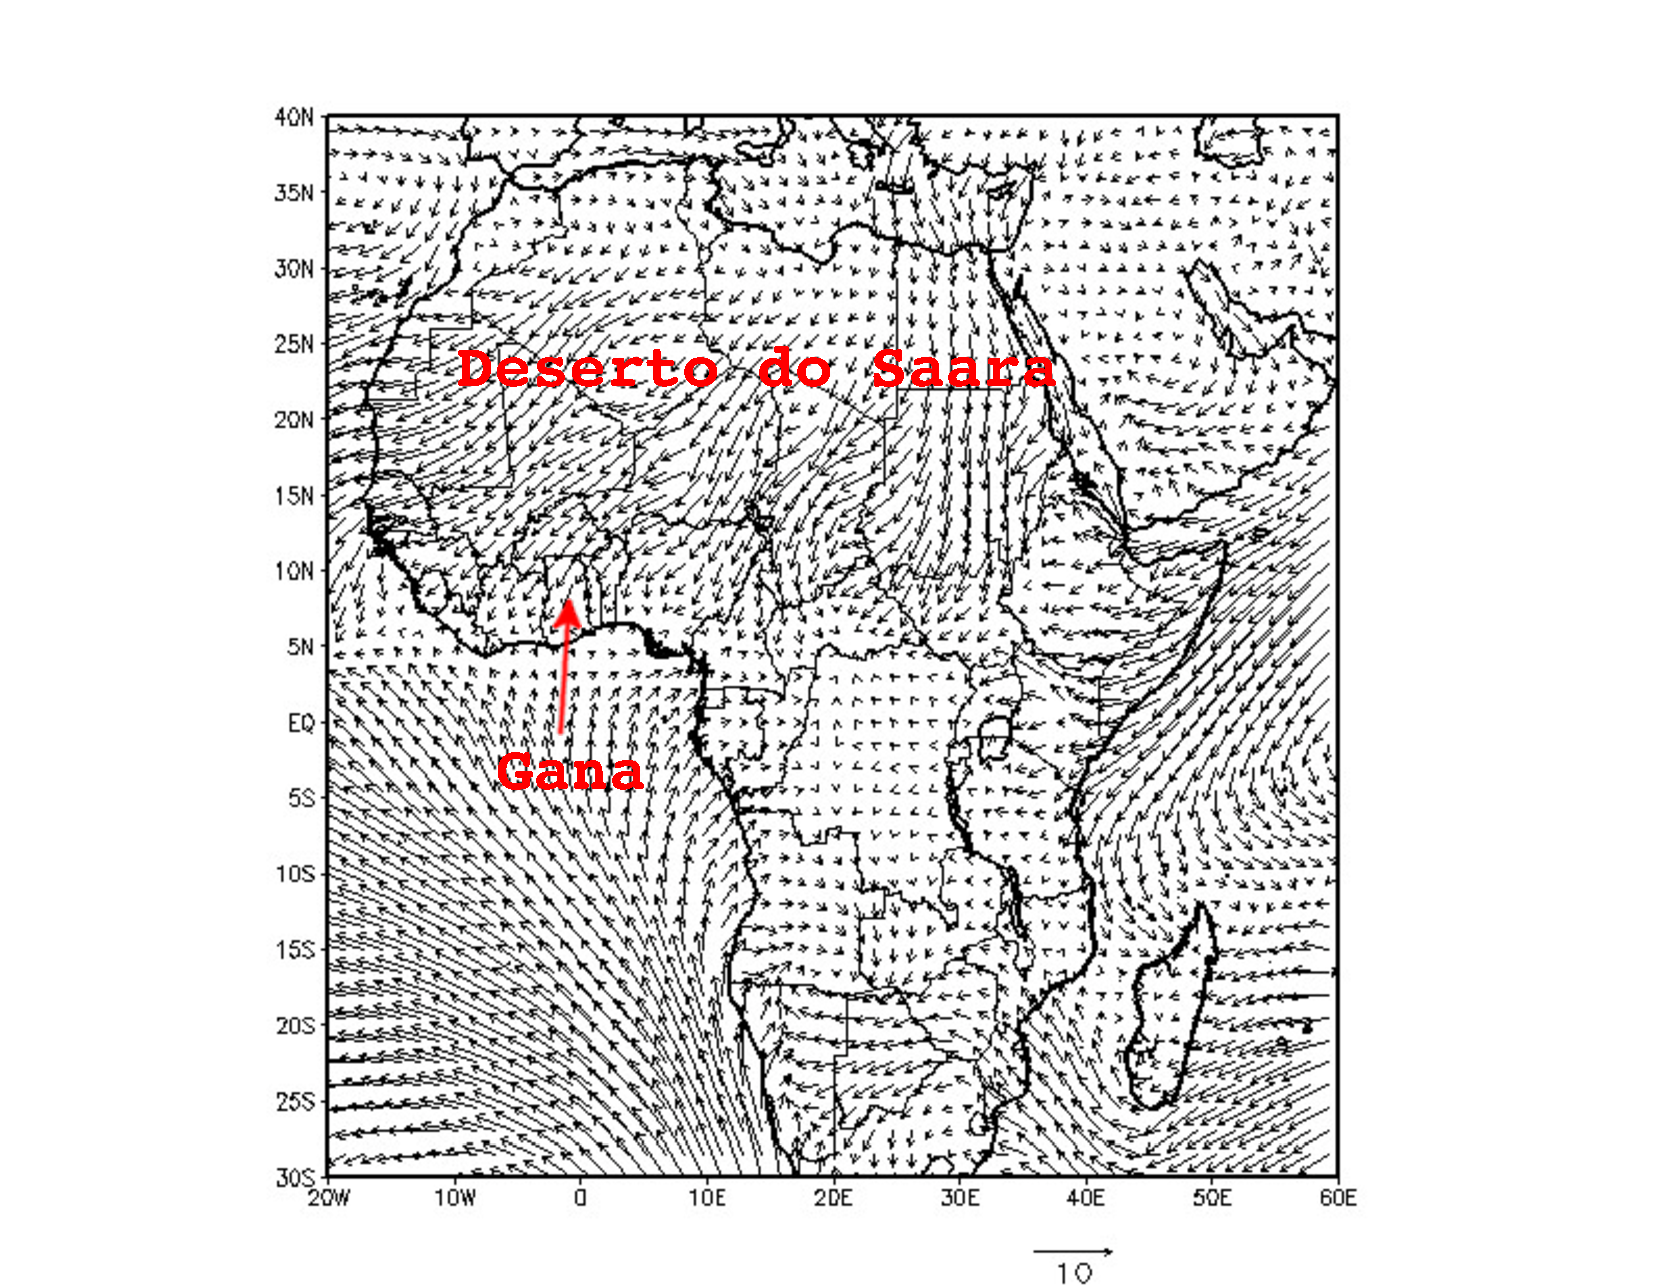
\includegraphics[width=\linewidth]{../../inputs/grads/gimp/1000hPa/JAN_2008.pdf}
      \caption{10 metros}
    \end{subfigure}%
  %  \hspace{0.5cm}
    \begin{subfigure}[b]{0.5\linewidth}
      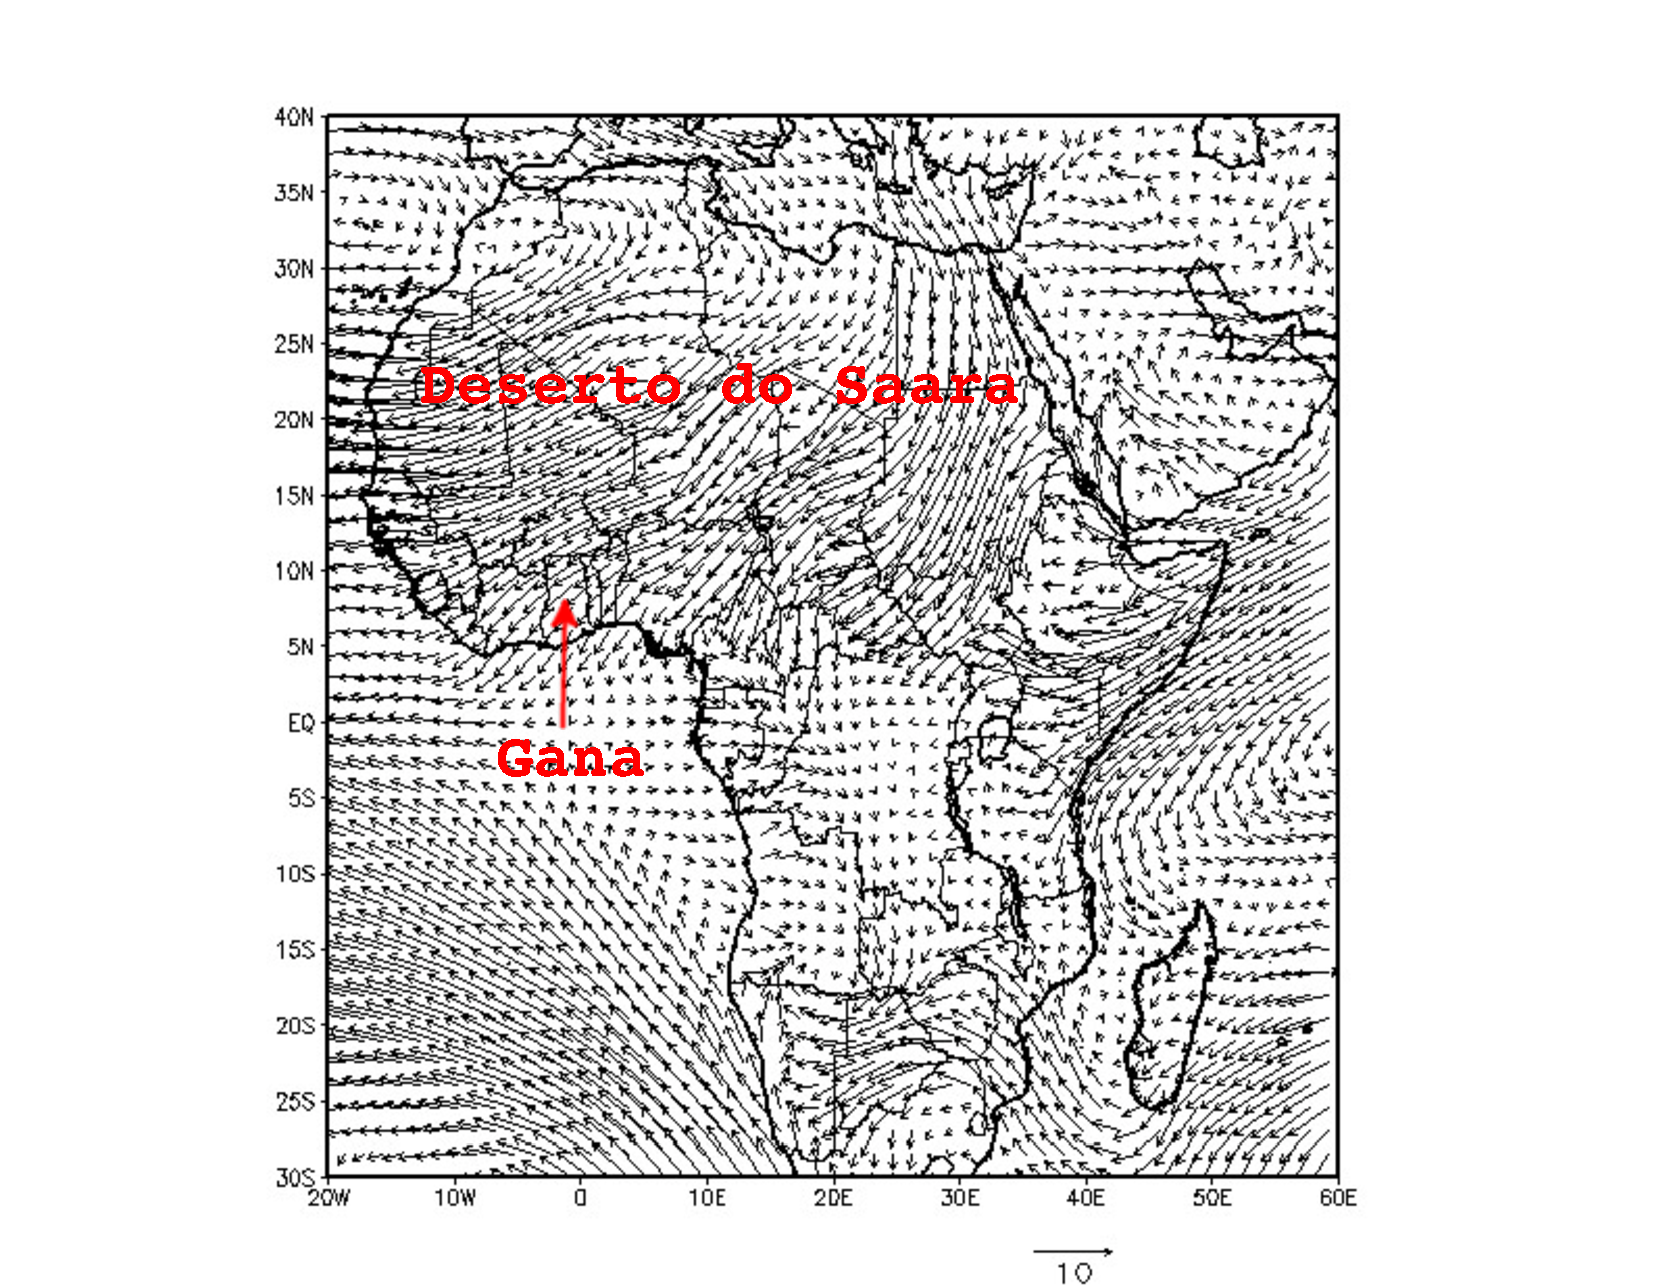
\includegraphics[width=\linewidth]{../../inputs/grads/gimp/875hPa/JAN_2008.pdf}
      \caption{1000 metros}
    \end{subfigure}
  \end{figure}
\end{frame}

\subsection{Identificaçao das fontes}



\begin{frame}
  \frametitle{}
  Análise de Fatores na área residencial para $MP_{2,5}$
               excluindo dias de ocorrência de vento Harmatão. n = 123.          
  \begin{table}[H]
    \centering
    \tiny
    \input{../../outputs/beautifulFAdisplay_RFsH5.tex}
  \end{table}
\end{frame}

\begin{frame}
  \frametitle{}
Análise de Fatores na avenida para $MP_{2,5}$
           excluindo dias de ocorrência de vento Harmatão. n = 122.         
  \begin{table}[H]
    \centering
    \tiny
    \input{../../outputs/beautifulFAdisplay_TFsH5.tex}
  \end{table}
\end{frame}



\begin{frame}
  \frametitle{}
    \begin{figure}
      \centering
            \begin{minipage}[b]{0.4\linewidth}
              \tiny
              \input{../../outputs/RFsH_profiles_percent_species5.tex}
      
            \end{minipage}
                  \hspace{3cm}
      \begin{minipage}[b]{0.3\linewidth}
        \includegraphics[width=\linewidth]{../../outputs/RFsH_pmf_contribution_pizza5.pdf}

      \end{minipage}%\hfill


    \end{figure}
\end{frame}


\begin{frame}
  \frametitle{}
  \begin{table}[H]
    \centering
    \tiny
    \begin{tabular}{llll|lll|ll|lll}
\hline
                                                  &                        & \multicolumn{5}{c|}{Residencial (massa média 27,52 $\mu g / m^3$)} & \multicolumn{5}{c}{Avenida (massa média 31,9 $\mu g / m^3$)}    \\
                                                  &                        & \multicolumn{2}{c}{AF}      & \multicolumn{3}{c|}{PMF}              & \multicolumn{2}{c}{AF}                      & \multicolumn{3}{c}{PMF}          \\
\hline
 & & & & \multicolumn{3}{c|}{contribuição na massa} & & & \multicolumn{3}{c}{contribuição na massa} \\
Fonte associada                                   & Elementos majoritários & $NF^1$   & VE$^2$ (\%)               & $NF^1$   & (\%)   & $\mu g / m^3$  & $NF^1$       & VE$^2$  (\%)            & $NF^1$ & (\%)  & $\mu g / m^3$ \\
\hline
\textbf{Solo}                                     & Mg,Al,Si,Ca,Ti,V,Mn,Fe & 1   & 43,78                 & 3   & 22,2         & \textbf{6,11}   & 1       & 45,49               & 3 & 22,2        & \textbf{7,08}  \\
\textbf{Queima biomassa}                          & P,S,K                  & 2   & 12,36                 & 5   & 21,6         & \textbf{5,94}   & 2       & 13,44               & 4 & 28,8        & \textbf{9,19}  \\
\textbf{Veículos}                                 & BC,Zn,K,Pb             & 3   & 11,24                 & 1   & 40,0           & \textbf{11,01}  & 5       & 7,19                & 5 & 31,5        & \textbf{10,05} \\
\textbf{Mar}                                      & Na,Cl                  & 4   & 8,81                  & 4   & 11,6         & \textbf{3,19}   & 3       & 9,76                & 2 & 13,6        & \textbf{4,34}  \\
\textbf{Queima lixo} & Br,Pb                      & 5   & 7,40                   & 2   & 4,65         & \textbf{1,28}   & 4       & 8,73                & 1 & 3,86        & \textbf{1,23} \\

\hline
\multicolumn{12}{l}{$^1$ NF: Número do Fator} \\
\multicolumn{12}{l}{$^2$ VE: Variância Explicada} \\
\hline
\end{tabular}


    \caption{Síntese das associações dos fatores extraídos na AF e PMF com fontes 
             poluidoras para $MP_{2,5}$. \label{sintese_fino}}
  \end{table}
\end{frame}


\begin{frame}
  \frametitle{}
\end{frame}



\begin{frame}
  \frametitle{}
\end{frame}


\begin{frame}
  \frametitle{}
\end{frame}



\begin{frame}
  \frametitle{}
\end{frame}



